
\documentclass[12pt]{article}
%\usepackage[T1]{fontenc}
\usepackage[utf8]{inputenc}
\usepackage[spanish]{babel}
\usepackage[pdftex]{graphicx}
\usepackage{authblk}
\newcommand{\HRule}{\rule{\linewidth}{0.5mm}}
\usepackage[breaklinks=true]{hyperref}
\hypersetup{
    colorlinks=true,
    linkcolor=black,
    filecolor=red,      
    urlcolor=blue,
    citecolor=cyan,
}

\usepackage{graphicx}
\usepackage{amsmath}
\usepackage{amssymb}
\usepackage{placeins} 
\usepackage{listings}
\usepackage{vmargin}
\usepackage{hyperref}
\usepackage{multirow}
\usepackage[table,xcdraw]{xcolor}
\usepackage{cite} % para contraer referencias


\usepackage{float}
\usepackage{graphicx}
\usepackage{url}
\usepackage{placeins}
\usepackage{subfigure}
\usepackage{multicol}
\usepackage{amsmath}
\usepackage{ulem}
\usepackage{blindtext}
\usepackage{enumitem}
\usepackage{tabularx}
\addtolength{\textwidth}{2cm}
\addtolength{\hoffset}{-1cm}
\setlength\parindent{0pt}
\setlength{\parskip}{0.5cm}


\usepackage{biblatex} %Imports biblatex package
\addbibresource{sample.bib} %Import the bibliography file

\begin{document}

%=====================================================================================

\pagenumbering{gobble}

%\input{./Cartaanteproyecto.tex}
%\clearpage\null\newpage

%\input{./cartatutor.tex}
%\clearpage\null\newpage

%\input{./cartatesis.tex}
%\clearpage\null\newpage

\begin{titlepage}
	\centering
	
\includegraphics[width=0.5\textwidth]{tb}\par\vspace{1cm}
	{\scshape\large Modelado y validación de Arquitectura para \textbf{TouresBalón} \par}
	\vspace{2cm}
	{ \textbf{Maestria en Ingeniería de Software}\par}
	\vspace{1.5cm}
	
	{ Diego Fernando Ochoa, Julian Osorio, Diana Carolina Mu\~noz Hurtado\par}
	\vspace{0.2cm}
	Profesor\\
	Alejandro Diaz Gutierres

	\vspace{2cm}
    
    {\bfseries Maestría en Ingener\'ia de Software \\
    Facultad de Ingenier\'ia\\
    Pontificia Universidad Javeriana - Cali\\
    \vspace{1.2cm}
    Mayo 2021\par}
    
\end{titlepage}
%\clearpage\null\newpage

%=====================================================================================

%\section*{Agradecimientos}




%\clearpage\null\newpage


%=====================================================================================
%\section*{Resumen}


\pagenumbering{gobble}
\newpage

%=====================================================================================
%\section*{Abstract}



%\pagenumbering{gobble}
%\newpage


\tableofcontents
\addtocontents{toc}{\hfill \textbf{Página} \par}

%\addtocontents{toc}{\hspace{-7.5mm} \textbf{Capítulos}}
%\addtocontents{toc}{\hfill \textbf{Página} \par}
\addtocontents{toc}{\vspace{-2mm} \hspace{-7.5mm} \hrule \par}







\newpage

\listoffigures

\newpage

%\listoftables

%\newpage

%=====================================================================================
%\section*{Prólogo}
\pagenumbering{arabic}

\pagenumbering{gobble}
\newpage


%=====================================================================================
\section{Presentación}



\pagenumbering{arabic}





%\newpage


%=====================================================================================
\subsection{Propósito del documento}

El actual proyecto surge a través de una necesidad, la cual es realizar un modelo de Arquitectura Empresarial del proceso de creación de planes turísticos para asistir a los espectáculos deportivos para la empresa \textbf{TouresBalon}, con la finalidad de poder cubrir las inconsistencias que existen entre los procesos, usuarios, stakeholders, etc., las mismas que ocasionan pérdida de recursos, tiempo, además de afectar directamente la reputación y seriedad de la compañía.

Así mismo, existe la necesidad de automatizar los procesos. De esta manera, gracias al desarrollo de la arquitectura empresarial para que el proceso de creación de planes turísticos para asistir a los espectáculos deportivos se puede optimizar y reducir los costos, gastos, tiempos utilizados actualmente en la entidad; lo cual genera no solo un cuello de botella en el procedimiento general si no perdidas de dinero por lentitud. Para ello, es necesario que los procesos a los que se recurren estén automatizado de igual manera sus entradas, flujo interno y salidas, de tal manera que, los tiempos sean acordes al proceso.  
%=====================================================================================
\subsection{Objetivos del Ejercicio de Arquitectura}

\subsubsection{Objetivo principal}
Realizar una propuesta de implementación de un modelo basado en las especificaciones del proyecto TouresBalón con marco de referencia TOGAF y un modelo  de vistas arquitecturales que busca mejora los procesos internos de la organización.

\subsubsection{Objetivos especificos}
\begin{itemize}
    \item Realizar el levantamiento y recopilación de la documentación necesaria del estado actual a través modelo organizacional de TOGAF.
    \item Realizar un análisis de negocio con cada uno de los elementos del sistema presente
    \item Proponer estrategias que mejoren los objetivos con respecto a rentabilidad y talento humano
    \item Establecer la arquitectura destino a la cual aspira la aplicación para TouresBalon
    \item Representar el modelo propuesto de TouresBalon, en el software “ARCHIMATE” desarrollado
    \item Definir los parámetros necesarios para la migración del estado actual de la arquitectura
\end{itemize}







%========================================================================

\subsection{Problema que se presenta }

Todos los procesos manuales y secuenciales generan perdidas en ventas por pedidos que se rechazan por que no son entregados a tiempo


%=====================================================================================

\subsection{Glosario}
\begin{itemize}
\item \textbf{Arquitectura de aplicaciones:} Define las funcionalidades siendo estos los servicios que brindan las aplicaciones

\item \textbf{Arquitectura de negocios:}  Es la arquitectura donde se identifica la línea base y la arquitectura final respecto al negocio.

\item \textbf{Arquitectura de tecnología:} Conjunto de acciones que realiza el área de TI en coordinación con la alta dirección para movilizar sus recursos de la forma más eficiente en respuesta a requisitos regulatorios, operativos o del negocio. 

\end{itemize}


%=====================================================================================



\section{Misión}
Con-fiabilidad, cumplimiento y competitividad; por la calidad de servicio que diariamente brindamos para lograr satisfacer las necesidades turísticas-

%=====================================================================================



\section{Visión}
A través de nuestro excelente portafolio de servicio, lograr un posicionamiento y un respeto en el mercado nacional como integrador de paquetes turísticos.




%=====================================================================================



\section{Modelo Motivacional}

En esta se sección se realiza el mapeo de todos los elementos del sistema presente, donde se proponen los objetivos estratégicos, metas y restricciones que permiten realizar un modelo arquitectural empresarial




%=====================================================================================


\subsection{Interesados} Se presenta el catalogo de interesados, en este caso se mantienen los mismos interesados del sistema presente y se representa el proceso motivacional en relación a los que se definen a continuación:

\begin{table}[H]
\centering
\begin{tabular}{|l|l|}
\hline
\textbf{Id} & \textbf{Interesados} \\ \hline
I1 & Gerente General \\ \hline
I2 & Gerente comercial \\ \hline
I3 & Gerente Logistica \\ \hline
I4 & Gerente admin \\ \hline
I5 & Director de sistemas \\ \hline
\end{tabular}
\end{table}



%\newpage

%=====================================================================================

\subsection{Preocupaciones} Se desarrollan las preocupaciones por interesados dados los elementos del sistema presente

\begin{table}[H]
\centering
\begin{tabular}{|l|l|l|}
\hline
\textbf{Id} & \textbf{Interesados} & \textbf{Preocupación} \\ \hline
I1 & Gerente General & Reducción de costos Aumento Rentabilidad \\ \hline
I2 & Gerente comercial & Reducción de tiempos en planes \\ \hline
I3 & Gerente Logística & Reducción de tiempos de entrega \\ \hline
I4 & Gerente Admon & Automatización de Procesos internos
\\ \hline
I5 & Director de sistemas & Plataforma Ágil 
\\ \hline
\end{tabular}
\end{table}





%=====================================================================================

\subsection{Objetivos}


\subsubsection{Objetivo de la arquitectura}

Establecer la situación actual de la arquitectura empresarial de TouresBalón y a través de la identificación del modelo motivacional, operacional, de capacidades y organizacional para determinar una arquitectura objetivo.


\subsubsection{Objetivos estratégicos y metas}

\begin{table}[H]
\centering
\resizebox{17cm}{!} {
\begin{tabular}{|l|l|l|}
\hline
\textbf{Id Objetivo} & \textbf{Descripción} & \textbf{Id Meta} \\ \hline
Obj 1 & Participar en los mercados con nuestros productos competitivos,  pero que sean beneficiosos para TouresBalón & M1 \\ \hline
Obj 2 & Generar crecimiento con Calidad de Servicio y Cumplimiento a nuestros clientes internos y externos & M2\\ \hline
Obj 3 & Permitirles a clientes internos  una importante  participación de lluvia de ideas, en las decisiones  y  mejoramientos  de estrategias  comerciales & M3 \\ \hline
Obj 4 & Reconocimiento de Marca, TouresBalónencontrará una solución ágil, con precio justo y confiable& M4 \\ \hline
\end{tabular}
}
\end{table}


\begin{itemize}
    \item M1 : Incrementar Convenios tecnológicos con aerolíneas y hoteles, aumentando el 50\% de convenido
    \item M2 : Mejorar la calidad de servicio aumentado el 80\% de efectividad en las transacciones de nuestros clientes
    \item M3 : Mejorar las estrategias comerciales a corto tiempo en un 30\%
    \item M4 : Incrementar el nombre de la marca en sus clientes en 75\% en sus clientes
\end{itemize}





%=====================================================================================


\subsection{Restricciones}
Se identifican las restricciones del sistema en general.

\begin{table}[H]
\centering
\begin{tabular}{|l|l|}
\hline
\textbf{Id} & \textbf{Restricciones} \\ \hline
I1 & El monto establecido por la Gerencia Comercial se actualiza mensualmente \\ \hline
I2 & Todo requerimiento técnico deberá ser evaluado por el líder del proyecto. \\ \hline
I3 & Monitoreo permanente en lineamientos y normatividad \\ \hline
\end{tabular}
\end{table}





%\newpage
%=====================================================================================

\subsection{Diagrama de modelo motivacional}

Para los gerentes del proyecto, se definen las motivaciones especificas y se relacionan los elementos definidos anteriormente en la figura 1:



\begin{figure}[ht]
\centering
\centering
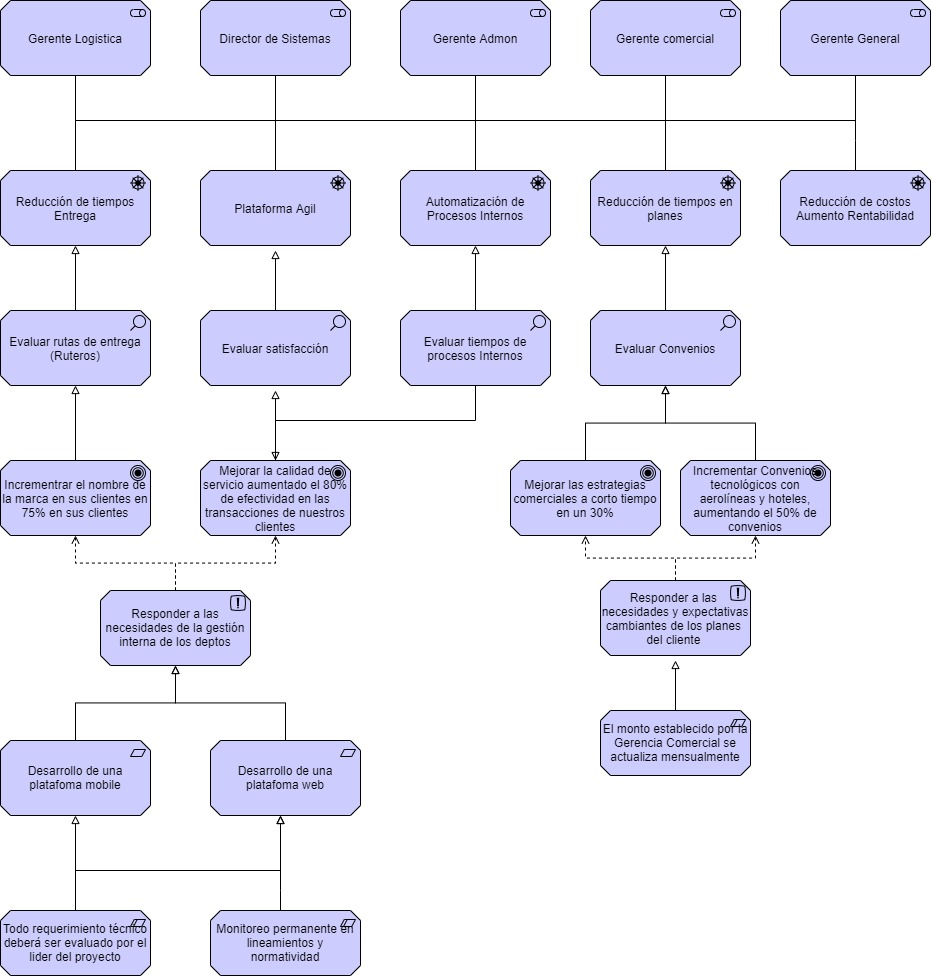
\includegraphics[scale=0.4]{imag/diagrama.jpeg}
\caption{Primer acercamiento de diagrama motivacional TouresBalón}
\label{1}
\end{figure}
\FloatBarrier









%=====================================================================================


\subsection{ Requerimientos}

\begin{itemize}
    \item Desarrollar una plataforma mobile.
    \item Desarrollar una plataforma web.
    \item La comunicación con Buses Bolivariano sobre de los viajes, sillas disponibles y reservas se debe realizar mediante archivos csv.
    \item La comunicación con Dann Carlton se debe realizar accediendo a un esquema de BD especial para TouresBalón.
\end{itemize}


%=====================================================================================


\subsection{Principios}

\begin{itemize}
    \item Responder a las necesidades, preferencias y expectativas cambiantes de los planes del  cliente
    \item Responder a las necesidades de la gestión interna de los departamentos.
\end{itemize}


%\newpage
%=====================================================================================
\section{Fast Track de Arquitectura empresarial}

\subsection{Negocio}

%=======================================================
\subsection{Modelo organizacional}

A continuación se describen los componentes del dominio de negocio que hacen parte del modelo organizacional de la empresa y cada una de las partes organizacionales. 

\begin{table}[H]
\centering
\resizebox{17cm}{!} {
\begin{tabular}{|l|l|l|}
\hline
\textbf{Código} & \textbf{Unidad} & \textbf{Descripción} \\ \hline
U01 & Unidad de Ventas & Unidad que se encarga de realizar las ventas dentro de la compañía \\ \hline
U02 & Unidad de Mercadeo & \begin{tabular}[c]{@{}l@{}}Unidad que se encarga del objetivo estratégico de la compañía, como \\ función principal es atender acciones para  proveer las necesidades del cliente\end{tabular} \\ \hline
U03 & Unidad de Transporte & \begin{tabular}[c]{@{}l@{}}Unidad que se encarga de administrar y gestionar los convenios  de \\ TouresBalón con las compañías de transporte\end{tabular} \\ \hline
U04 & Unidad de Hospedaje & \begin{tabular}[c]{@{}l@{}}Unidad que se encarga de administrar y gestionar los convenios de \\ TouresBalón con los diferentes tipos de Hospedaje\end{tabular} \\ \hline
U05 & Unidad de Espectaculos & \begin{tabular}[c]{@{}l@{}}Unidad que se encarga de administrar y gestionar los convenios con \\ las proveedoras encargadas de espectáculos\end{tabular} \\ \hline
U06 & Unidad Financiera & Unidad que se encarga de controlar el capital de la compañía \\ \hline
U07 & Unidad RRHH & \begin{tabular}[c]{@{}l@{}}Unidad que se encarga de la función de recursos humanos \end{tabular} \\ \hline
U08 & Unidad de Sistemas & Unidad que se encarga de proveer información a funciones específicas \\ \hline
\end{tabular}
}
\end{table}

\subsubsection{Organigrama}

El siguiente diagrama nos permite tener una visión general de la infraestructura de la organización:

\begin{figure}[ht]
\centering
\centering
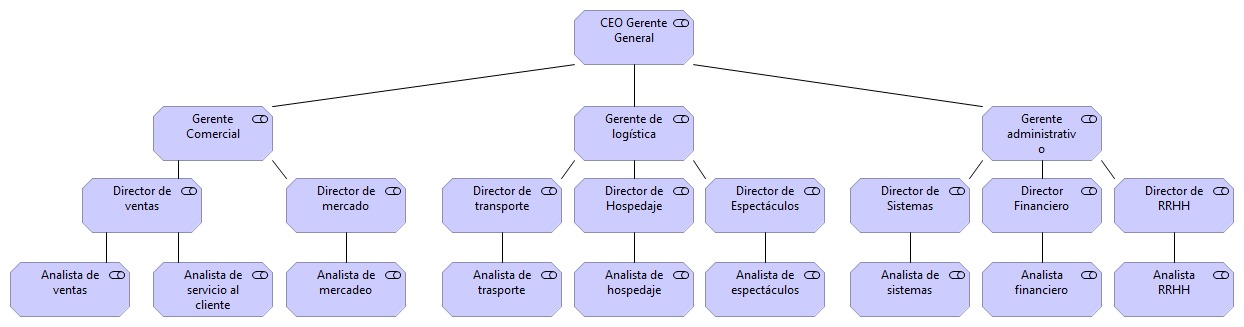
\includegraphics[scale=0.4]{organi.jpeg}
\caption{Organigrama base de la compañía}
\label{2}
\end{figure}
\FloatBarrier






\subsubsection{Catalogo de unidades organizacionales }
\subsubsection{Catalogo de roles}

\begin{table}[H]
\centering
\resizebox{17cm}{!} {
\begin{tabular}{|l|l|l|}
\hline
\textbf{Código} & \textbf{Rol} & \textbf{Descripción} \\ \hline
R01 & Gerente general & Unidad que se encarga de realizar las ventas dentro de la compañía \\ \hline
R02 & Gerente Comercial & \begin{tabular}[c]{@{}l@{}}Unidad que se encarga del objetivo estratégico de la compañía, como \\ función principal es atender acciones para  proveer las necesidades del cliente\end{tabular} \\ \hline
R03 & Gerente de Logistisca & \begin{tabular}[c]{@{}l@{}}Unidad que se encarga de administrar y gestionar los convenios  de \\ TouresBalón con las compañías de transporte\end{tabular} \\ \hline
R04 & Director de ventas & \begin{tabular}[c]{@{}l@{}}Unidad que se encarga de administrar y gestionar los convenios de \\ TouresBalón con los diferentes tipos de Hospedaje\end{tabular} \\ \hline
R05 & Director de transporte & \begin{tabular}[c]{@{}l@{}}Unidad que se encarga de administrar y gestionar los convenios con \\ las proveedoras encargadas de espectáculos\end{tabular} \\ \hline
R06 & Director Financiero & Unidad que se encarga de controlar el capital de la compañía \\ \hline
R07 & Director de Mercadeo & \begin{tabular}[c]{@{}l@{}}Unidad que se encarga de la función de recursos humanos \\ compuesta por áreas de reclutamiento, selección, contratación, capacitación, \\ administración del personal durante la permanencia en la empresa\end{tabular} \\ \hline
R08 & Director de Hospedaje & Unidad que se encarga de proveer información a funciones específicas \\ \hline
R09 & Director de RRHH & \begin{tabular}[c]{@{}l@{}}Es el encargado de funciones propias de reclutamiento, selección, \\ contratación, capacitación, administración del personal durante la permanencia \\ en la empresa\end{tabular} \\ \hline
R10 & Director de Espectaculos & \begin{tabular}[c]{@{}l@{}}Es el encargado de asegurar la realización de las actividades de espectáculo \\ ofrecidas por la compañía\end{tabular} \\ \hline
R11 & Director de Sistemas & \begin{tabular}[c]{@{}l@{}}Es el encargado de la validación y distribución de la información \\ en los procesos TI de la compañía\end{tabular} \\ \hline
\end{tabular}
}
\end{table}


%=======================================================
\subsection{Modelo operativo}
%\subsubsection{Diagrama de procesos nivel 2}
\subsubsection{Catalogo de procesos}

\begin{table}[H]
\centering
\resizebox{17cm}{!} {
\begin{tabular}{|l|l|l|}
\hline
\textbf{Catalogo de Procesos} & \textbf{Proceso} & \textbf{Descripción} \\ \hline
\textbf{P1} & Gestion Pedidos & Macroproceso que agrupa los procesos de gestion de pedidos \\ \hline
P1.1 & Validar Orden & Proceso que se encarga de verificar el producto \\ \hline
P1.2 & Verifico el inventario & Proceso que se encarga de revisar el inventario despues de validar el pedido \\ \hline
\textbf{P2} & Gestion Cliente & Macroproceso que agrupa los procesos de gestión de clientes \\ \hline
P2.1 & Valido el cliente & Proceso que se encarga de validar el usuario \\ \hline
P2.2 & Valido el pago & Proceso que se encarga de validar el pago del producto \\ \hline
\textbf{P3} & Gestion Contable & Macroproceso que agrupa los procesos de gestión de contabilidad \\ \hline
P3.1 & Facturo el Pedido & Proceso que se encarga de registrar la facturación del pedido \\ \hline
P3.2 & Descargo el Inventario & \begin{tabular}[c]{@{}l@{}}Proceso que se encarga de guardar el inventario de los \\ productos de la empresa\end{tabular} \\ \hline
P3.3 & Contabilizo inventario & \begin{tabular}[c]{@{}l@{}}Proceso que se encarga de llevar la contabilidad de los productos \\ que quedan después de los gastos y pagos\end{tabular} \\ \hline
\textbf{P4} & \textbf{Gestionar Recursos} & Macroproceso que agrupa los procesos de gestión de recursos \\ \hline
P4.1 & Valido ingreso & Proceso que se encarga de validar los ingresos por recurso \\ \hline
P4.2 & Valido venta & Proceso que se encarga de validar la venta por recurso \\ \hline
\end{tabular}
}
\end{table}


\subsubsection{Proceso de compra Nivel 1}
Se identifican los procesos detallados de compra


\begin{figure}[ht]
\centering
\centering
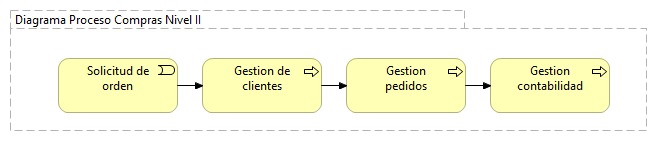
\includegraphics[scale=0.6]{pc2.jpeg}
\caption{Proceso de compra}
\label{2}
\end{figure}
\FloatBarrier

\begin{table}[H]
\centering
\resizebox{17cm}{!} {
\begin{tabular}{|l|l|l|}
\hline
\textbf{Proceso de compras} & \textbf{Nombre} & \textbf{Descripción} \\ \hline
\textbf{1} & El cliente reaiza el pedido &  \\ \hline
2 & Se crea el pedido &  \\ \hline
3 & Se valida que le pedido se pueda facturar &  \\ \hline
\textbf{4} & Se valida al cliente &  \\ \hline
5 & Se valida el pago &  \\ \hline
6 & Se Realiza verificación Logistico &  \\ \hline
\textbf{7} & Se Realiza separación paquete & Paquete: Hotel, vuelo, comidas, entradas al partido \\ \hline
8 & Se realiza pago de la separación &  \\ \hline
9 & Se realiza contabilización &  \\ \hline
10 & Se realiza encuentas de satisfacion cliente &  \\ \hline
\end{tabular}
}
\end{table}


\subsubsection{Proceso de compra Nivel 2}

\begin{figure}[ht]
\centering
\centering
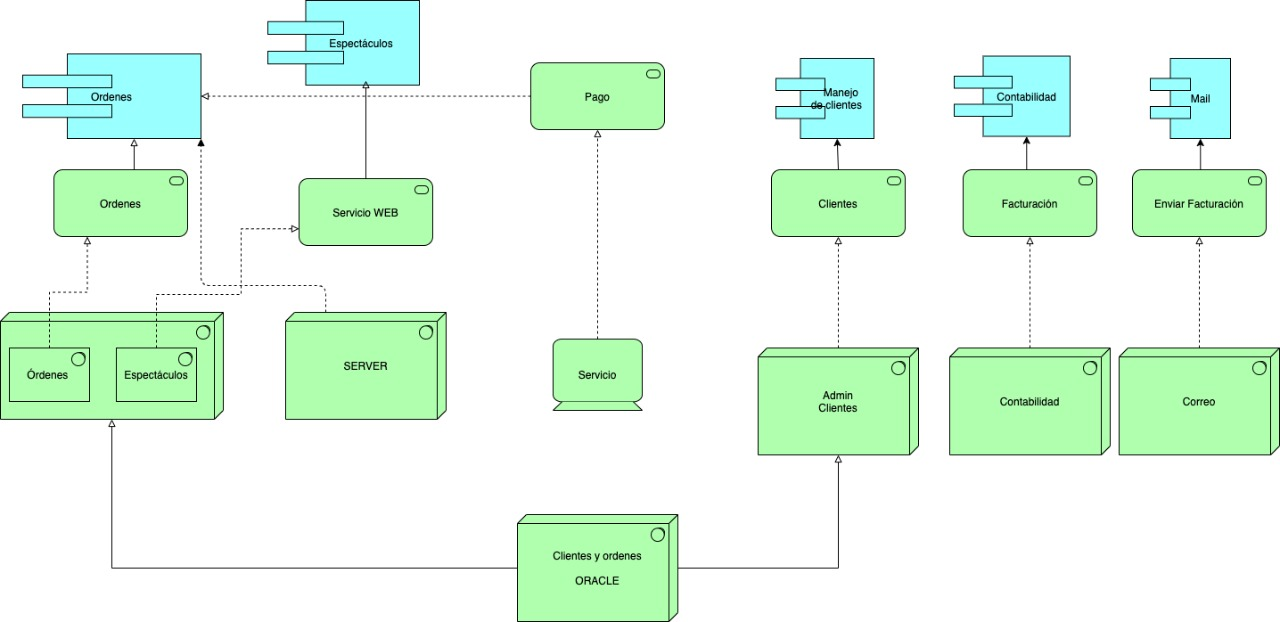
\includegraphics[scale=0.4]{Procesogeneral.jpeg}
\caption{Proceso de compra}
\label{2}
\end{figure}
\FloatBarrier



%=======================================================
\subsection{Modelo de capacidades}
Se identifican las capacidades del negocio, un elemento fundamental que nos permite construir el modelo organizacional.

\begin{table}[H]
\centering
\resizebox{17cm}{!} {
\begin{tabular}{|l|l|l|}
\hline
\textbf{Modelo de Capacidades} & \textbf{Nombre} & \textbf{Descripción} \\ \hline
\textbf{1} & Administracion de Convenios & Construir Mejores Convenio \\ \hline
 &  & Modificar Convenio propuestos \\ \hline
 &  & Eliminar Convenio actuales \\ \hline
\textbf{2} & Administracion de RRHH & Contratar Empleados \\ \hline
 &  & Despedir Empleados \\ \hline
 &  & Fidelizar empleado \\ \hline
\textbf{3} & Administracion Financiera & Contabilizar Documentos Compañia \\ \hline
 &  & Realizar Informes de la compañía \\ \hline
 &  & Cuidar Recursos Financieros de la empresa \\ \hline
\textbf{4} & Administración Comercial & Cumplir el presupuesto de ventas \\ \hline
\textbf{} &  & Fidelizar clientes \\ \hline
\textbf{5} & Administracion de Tecnologia & Mejorar procesos de la compañia al menor costo \\ \hline
 &  & Proponer avances de infraestructura \\ \hline
 &  & Proponer mejoras en la informacion oportuna \\ \hline
\end{tabular}
}
\end{table}

\subsubsection{Mapa de capacidades}


\subsubsection{Catálogo de capacidades}

\begin{table}[H]
\centering
\resizebox{10cm}{!} {
\begin{tabular}{|l|l|}
\hline
\textbf{Catálogo de Capacidades} & \textbf{Descripción} \\ \hline
\textbf{1} & Administración de Convenios \\ \hline
2 & Administración de RRHH \\ \hline
3 & Administración Financiera \\ \hline
\textbf{4} & Administración Comercial \\ \hline
5 & Administracion de Tecnologia \\ \hline
\end{tabular}
}
\end{table}





%=======================================================
\subsection{Datos}




\subsubsection{Catálogo de entidades conceptuales}

\begin{table}[H]
\centering
\resizebox{17cm}{!} {
\begin{tabular}{|l|l|l|}
\hline
\textbf{Catálogo de entidades Conceptuales} & \textbf{Nombre} & \textbf{Descripción} \\ \hline
\textbf{1} & Pedidos & Documento con el cual se realiza la solicitud del cliente \\ \hline
2 & Factura & Documento de legazacion del pedido relalizado \\ \hline
3 & Tarifa Transporte & Valor por el servicio de transporte \\ \hline
\textbf{4} & Tarifa Hospedaje & Valor del hospedaje \\ \hline
5 & Tarifa Comida & Valor de la comida \\ \hline
6 & Margen Utilidades & Valor de la utilidad por la venta \\ \hline
7 & Fidelizacion & Proceso con la finalidad de mantener el cliente para una próxima solicitud \\ \hline
8 & Inventario & Capacidad de ventas por evento \\ \hline
9 & Empleados & Recurso disponible de la empresa para realizar labor encomendada \\ \hline
10 & Departamento & Asignación de responsabilidades dentro de la compañía \\ \hline
11 & Ciudad & Destino de solicitud \\ \hline
\end{tabular}
}
\end{table}



\subsubsection{Diagrama conceptual de datos}
\begin{figure}[ht]
\centering
\centering
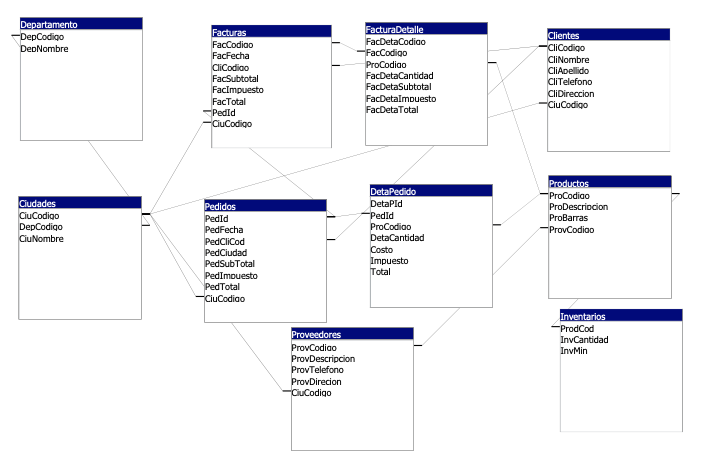
\includegraphics[scale=0.6]{Diagrama de datos.png}
\caption{Diagrama de datos}
\label{2}
\end{figure}
\FloatBarrier






%=======================================================
\subsection{Atributos de calidad}
\begin{table}[H]
\centering
\resizebox{6cm}{!} {
\begin{tabular}{|l|l|}
\hline
\textbf{No} & \textbf{Atributo de Calidad} \\ \hline
\textbf{1} & Disponibilidad \\ \hline
2 & Performance \\ \hline
3 & Seguridad \\ \hline
\end{tabular}
}
\end{table}

\subsubsection{Escenarios de Arquitectura}
\input{./ESc01.tex}

\input{./ESc02.tex}

\input{./ESc03.tex}

\input{./ESc04.tex}

\input{./ESc05.tex}


\subsection{Tácticas del sistema}

\begin{table}[H]
\centering
\resizebox{17cm}{!} {
\begin{tabular}{|l|l|}
\hline
\textbf{Atributo de Calidad} & Táctica de Arquitectura \\ \hline
\textbf{Seguridad} & Usuario ingreso con sus credenciales correctas \\ \hline
Disponibilidad & \begin{tabular}[c]{@{}l@{}}Tolerancia a fallos, el sistema debe permanecer el \\ mayor tiempo posible, uso de watchdog\end{tabular} \\ \hline
Performance & La aplicación \\ \hline
\end{tabular}
}
\end{table}


%=======================================================
\subsection{Vista de aplicación propuesta infraestructura software TouresBalón}

Se propone la metodología C4 para la visualización de la arquitectura de software, este modelo nos permite ilustrar el contexto y sus relaciones funcionales en contenedores y componentes 

\subsubsection{Nivel C1 de contexto}

En este nivel nos enfocamos en extraer la información planteada del sistema.

\begin{figure}[ht]
\centering
\centering
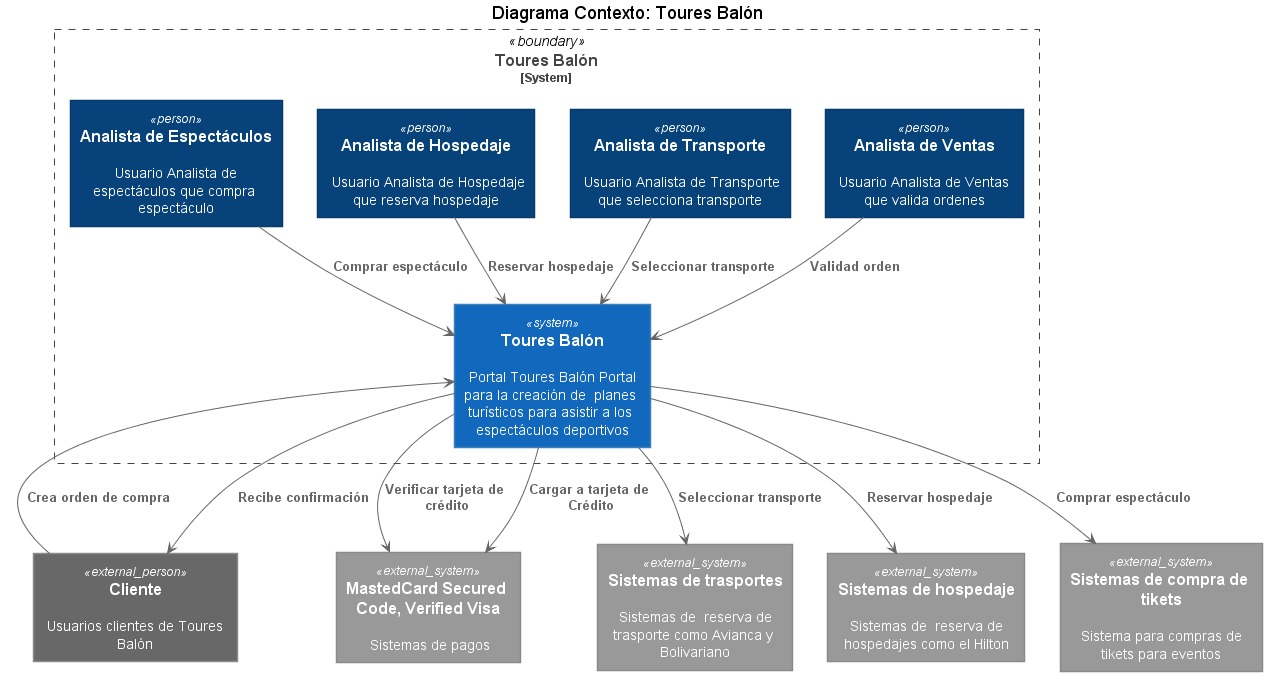
\includegraphics[scale=0.4]{DC.jpeg}
%\caption{Propuesta infraestructura software TouresBalón}
\label{2}
\end{figure}
\FloatBarrier

\subsubsection{Nivel C2 Diagrama de contenedores}

En este nivel nos enfocamos en desarrolla el modelo contenedores de la compañía, como una representación de la aplicación y sus unidades ejecutables.


\begin{figure}[ht]
\centering
\centering
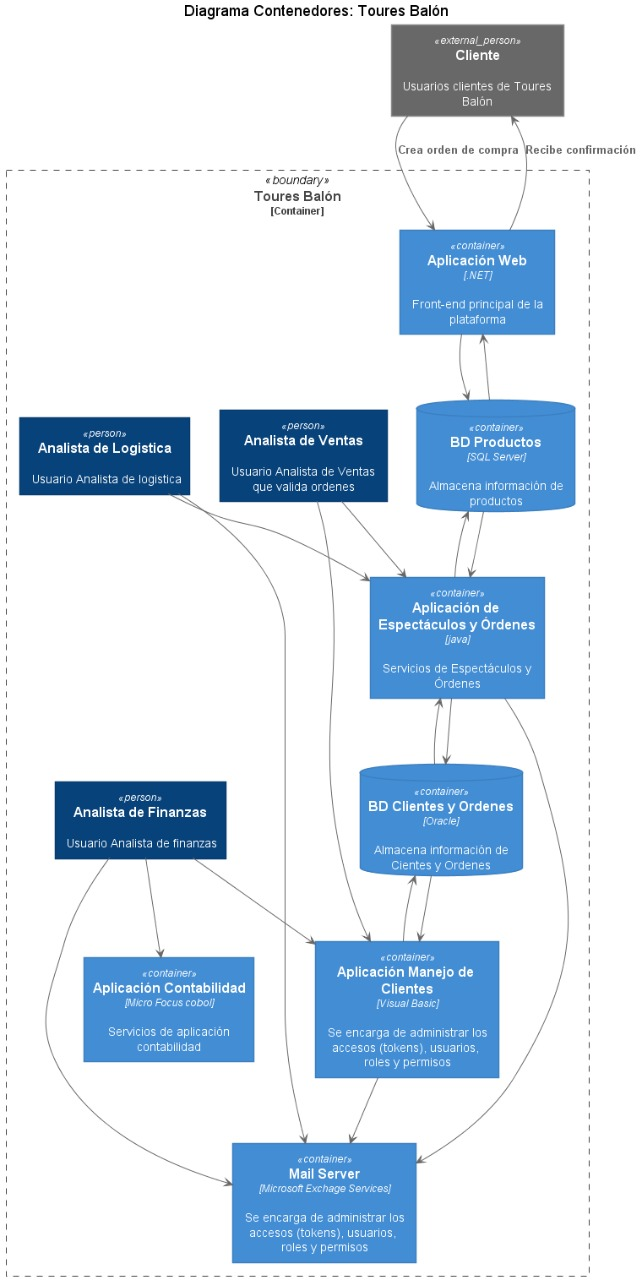
\includegraphics[scale=0.4]{Diagrama de contenedores.jpeg}
%\caption{Propuesta infraestructura software TouresBalón}
\label{2}
\end{figure}
\FloatBarrier


\subsubsection{Nivel C3 Diagrama de componentes}
En este nivel nos enfocamos en descomponer cada contenedor más para identificar los principales bloques de construcción estructural y sus interacciones. El diagrama de componentes muestra cómo un contenedor se compone de una serie de componentes, cuáles son cada uno de esos componentes, sus responsabilidades y los detalles de implementación.

\begin{figure}[ht]
\centering
\centering
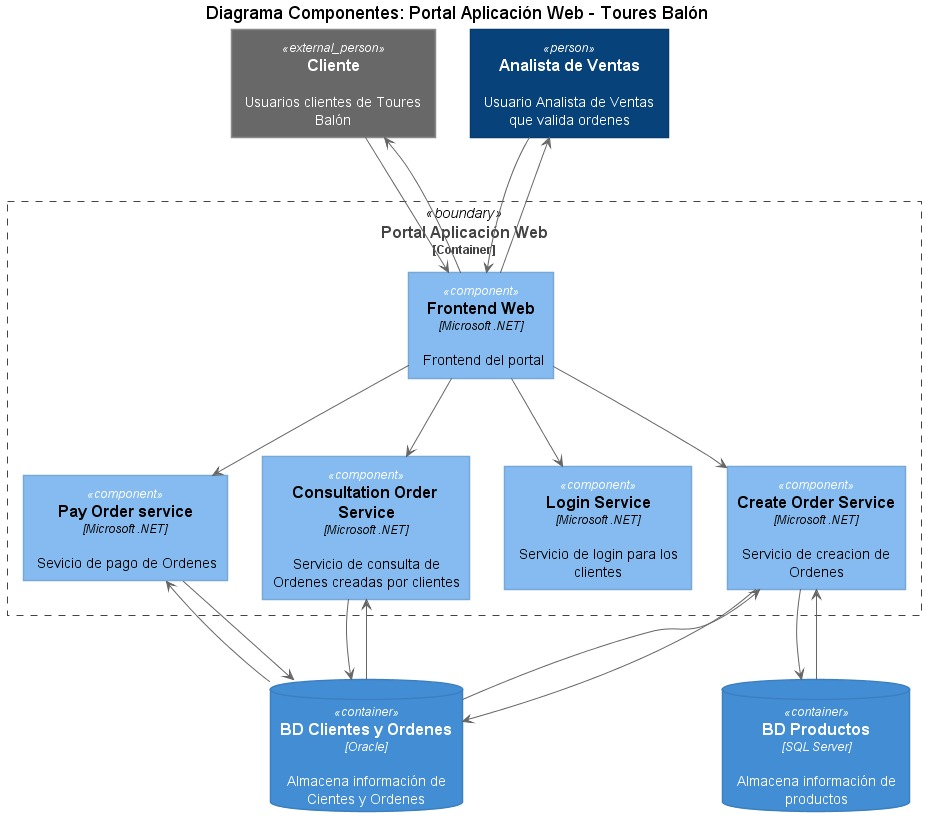
\includegraphics[scale=0.4]{C3.jpeg}
%\caption{Propuesta infraestructura software TouresBalón}
\label{2}
\end{figure}
\FloatBarrier


%=======================================================
\subsection{Vista de tecnología propuesta infraestructura software TouresBalón}

Se propone la metodología C4 para la visualización del diagrama de despliegue , este modelo nos permite ilustrar el contexto y sus relaciones funcionales en contenedores y componentes 

\subsubsection{Diagrama de despliegue (deployment) implementación}

En este nivel nos enfocamos en el diagrama de implementación que nos permite ilustrar cómo los sistemas de software y / o contenedores en el modelo estático se asignan a la infraestructura.


\begin{figure}[ht]
\centering
\centering
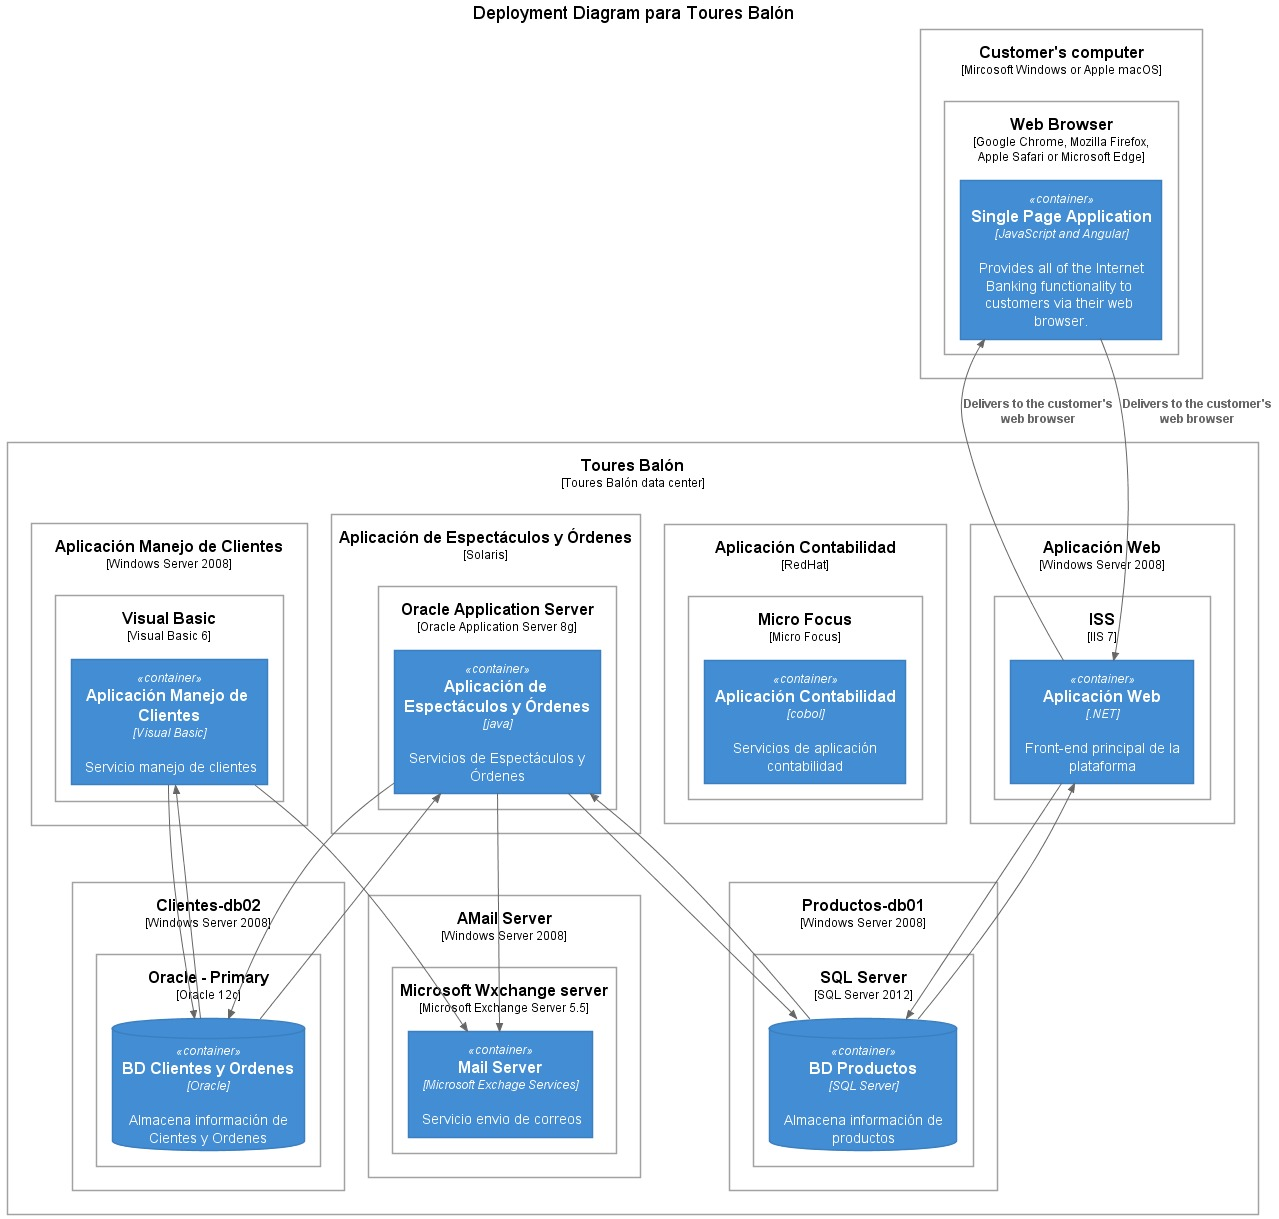
\includegraphics[scale=0.4]{C4.jpeg}
%\caption{Propuesta infraestructura software TouresBalón}
\label{2}
\end{figure}
\FloatBarrier




%=======================================================
%\subsection{Aplicaciones}
%\subsubsection{Vista de estructura de aplicaciones}
%\subsubsection{Vista de cooperación de aplicaciones}
%\subsubsection{Catálogo de aplicaciones}
%\subsubsection{Matriz de aplicaciones vs aplicaciones}

%=======================================================
%\subsection{Tecnología}
%\subsubsection{Vista de uso de infraestructura}
%\subsubsection{Catalogo de componentes de tecnología}
%\subsubsection{Catalogo de servicios de tecnología}



%=======================================================
\subsection{Conclusiones}
\begin{itemize}
    \item Estudiar los pasos de construir un modelos de arquitectura empresarial nos permite identificar las características clave para modelar un sistema deseado.
    
    \item Las empresas requieren de instrumentos que les permitan una mayor agilidad empresarial, la cual es posible si se facilita la implantación de nuevos modelos de negocio de forma rápida y la obtención de una mejora en la eficiencia empresarial, utilizar los procesos adecuados para la implementación del sistema nos ahorra tiempo y costos.
    
    \item El desarrollo de la Arquitectura tanto empresarial como de software se debe entender como la descripción integral y estructurada de los diferentes elementos que conforman el sistema de la empresa.
\end{itemize}












%%%%%%%%%%%%%%%%%%%%%%%%%%%%%
% BIBLIOGRAFIA
%%%%%%%%%%%%%%%%%%%%%%%%%%%%%
%\bibliography{biblio.bib}
%\bibliographystyle{IEEEtran}
%\notice{1}


%%%%%%%%%%%%%%%%
% GENERAL INDEX
%%%%%%%%%%%%%%%%
%\printindex



%\section{Anexos}




\end{document}


